\section{训练}
\noindent 1、优化器和损失函数的设置: 使用随机梯度下降 (SGD) 作为优化器,学习率为 0.01。
使用交叉熵损失函数 (CrossEntropyLoss)。\\
\noindent 2、训练循环:设置了总共 100 个训练周期 (epochs)。
在每个周期内,遍历训练数据集,并进行前向传播、反向传播和优化。
输出每个步骤的训练进度信息,包括当前周期和步骤。\\
\noindent 3、模型保存:在训练完成后,将模型保存到文件 'model/model.pth'。\\
\noindent 4、损失和准确率的记录:记录每个训练周期的总损失和准确率。
绘制训练损失和准确率随着训练周期变化的图表。\\
\noindent 5、100个轮次训练结果为:总损失803.9553998112679,准确率0.9351993865030674
\noindent 图像如下:
\begin{figure}[H]
	\centering
	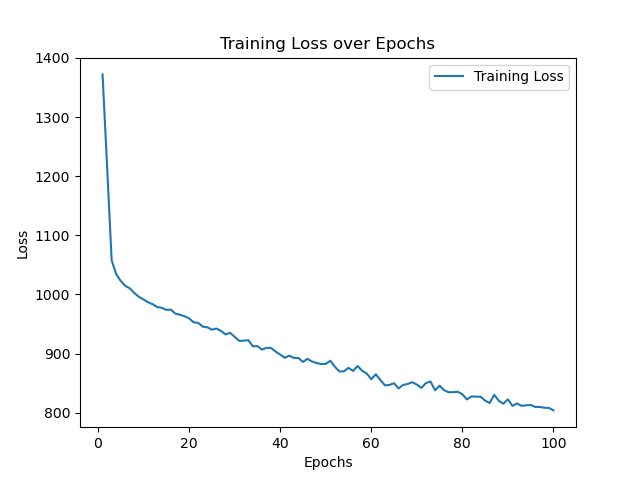
\includegraphics[width=0.7\textwidth]{loss_plot.png}
	\caption{损失值随训练轮次变化}
	\label{fig:example}
\end{figure}

\begin{figure}[H]
	\centering
	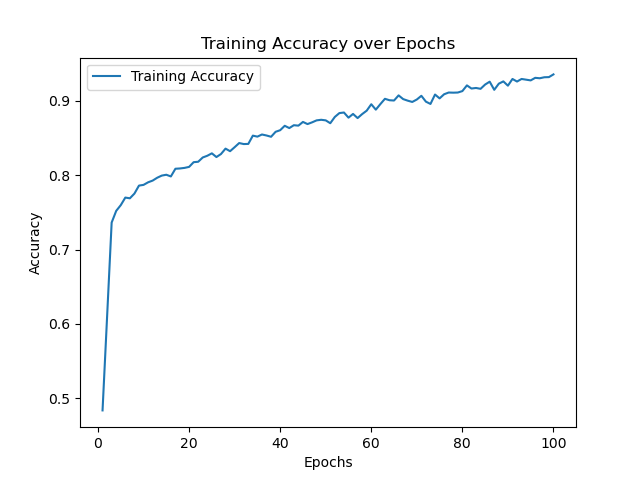
\includegraphics[width=0.7\textwidth]{accuracy_plot.png}
	\caption{准确率随训练轮次变化}
	\label{fig:example}
\end{figure}